\documentclass[10pt]{article}
\makeindex
\usepackage{amsmath, amsfonts, amssymb, amstext, amscd, amsthm, graphicx,makeidx, hyperref, url, pgfplots, mathrsfs, mathtools}
\graphicspath{ {./images/} }
\pgfplotsset{width=7cm,compat=1.8}
\usepackage[margin=1.0in, headheight=40pt]{geometry}
\usepackage{fancyhdr}
\usepackage[english]{babel}
\usepackage[utf8]{inputenc}

\usepackage{caption}
\usepackage{subcaption}

\makeatletter
\renewcommand*\env@matrix[1][*\c@MaxMatrixCols c]{%
  \hskip -\arraycolsep
  \let\@ifnextchar\new@ifnextchar
  \array{#1}}
\makeatother

\allowdisplaybreaks
\newcommand{\R}{\mathbb{R}}
\newcommand{\C}{\mathbb{C}}
\newcommand{\Z}{\mathbb{Z}}
\newcommand{\N}{\mathbb{N}}
\newcommand{\Q}{\mathbb{Q}}
\newcommand{\F}{\mathbb{F}}
\newcommand{\ddx}{\frac{d}{dx}}

\pagestyle{fancy}
\fancyhf{}
\cfoot{\thepage}
\lhead{Alvin On\\
	  Nathan Suri\\
	  Laura Lewis
}
\chead{CS 101-3}
\rhead{Due Date: 6/6/2020}
\begin{document}
\begin{center}
\section*{Wave Function Collapse Project}
\end{center}

\section{Project Description}
We proposed our own project, based on the WaveFunctionCollapse algorithm, which can be seen \href{https://github.com/mxgmn/WaveFunctionCollapse}{here}. The original algorithm is a procedural generation algorithm to generate bitmaps that are locally similar to the input bitmap. The general idea is that based on this input bitmap, we are given a set of states (tiles) with neighboring constraints as input, where we want to randomly generate a larger board of a given size that satisfies the neighboring constraints from this. The original algorithm is based on quantum mechanics, where it initializes all tiles in a superposition of all states in the input and then observes the tile with the lowest entropy to collapse it. Following this, the changes caused by the collapse are propagated through the rest of the board until all constraints are satisfied. This repeats until all tiles are collapsed into a single state, in which we have the board we wanted to generate.\\
\indent Given this clear underlying quantum structure to the problem, our main goal is to incorporate our knowledge of quantum programming and algorithms from this course into the project, replacing certain parts of the algorithm with quantum ideas rather than this classical simulation of it. We aimed to do so in two different ways.\\
\indent The first was to keep the mainly classical approach to the algorithm and analyze the effect of utilizing a quantum random number generator to select the state for collapse. In the original algorithm, this state is selected using numpy's random.choice function. However, we were interested in seeing what difference, if any, it would make to adjust this to use a quantum random number generator. Furthermore, this was the first step in allowing us to begin incorporating more quantum ideas into the algorithm. To implement this, we did so in Q$\#$, where we generated a single random bit by applying the Hadamard gate to a qubit in the zero state. This causes the qubit to be in an equal superposition, such that upon measuring in the computational basis, we obtain a completely random result. Thus, we then obtained a random bit string by concatening many of these random bits, which we converted into an integer to obtain our final random integer to pass to the classical program. Furthermore, the classical program itself is largely a Python version of the original algorithm, which we will discuss in the Implementation section.\\
\indent Our second method for incorporating quantum computation into the WaveFunctionCollapse algorithm was through an algorithm similar to VQE from lecture. From our input image, we obtain frequencies for each of the tiles as well as a table of constraints on neighboring tiles. We then pass these frequencies into the quantum circuit, where the states are then encoded as one-hot vectors with each tile in superposition with the respective probabilities of being in each state as the amplitudes. Furthermore, by using a variational appproach, we can then arrive at the correct entanglement scheme in order to obain a board where the constraints are satisfied. This involves a quantum and classical hybrid algorithm very similar to VQE. Our idea for this is to have a parameterized quantum circuit, which strongly entangles the tiles and counts the number of conflicts with the constraints found earlier. In addition, this quantum circuit only deals with a section of the board at a time, given a center tile, the one to its right, and the one below it, when thinking about the arrangement of the board. Thus, we start from the top left tile and progressively apply the quantum circuit and count the number of conflicts for every possible center tile. Furthermore, we can pass this count to the classical machine in which we have a loss function that sums the total number of conflicts for the whole board. Our classical minimizer then selects new frequencies for the tiles, where this choice should minimize the number of conflicts that occur. Finally, when this minimizer converges on the board with the minimal number of conflicts with the constraints, we have the board we want.

\newpage
\section{Implementation}
\indent First, we will detail the quantum random number generation portion of the algorithm and how it fits in to the original classical WaveFunctionCollapse algorithm. The logic behind this implementation is that we replace the numpy call to choose a random initial position and random state to collapse with our quantum random number generator. In this method, we leave most of the original WaveFunctionCollapse algorithm as classical but then add in this small quantum element to see how it affects the runtime or results. The implementation of the random number generator is as follows. We use the Hadamard gate to put a qubit in an equal superposition and then measure this in the computational basis. Because the $|+\rangle$ state is an equal superposition of the computational basis states, measuring it will result in a perfectly random bit. Furthermore, we then loop to create a bit string made from concatenating these random bits together and convert this into an integer. Thus, we have obtained a random integer using quantum random number generation. Furthermore, we can assert an upper bound on the random number generated by only creating bit strings of a certain length and repeating this process until arriving at a suitable integer. Using this quantum technique for generating random integers, we then choose state in the wave function that we want to collapse as well as our initial state using this random number generator rather than the classical numpy ones. \\
\indent Now, we will discuss the variational approach to incorporating quantum computation into the WaveFunctionCollapse algorithm. As discussed earlier, the general idea for this implementation is to adapt the classical WaveFunctionCollapse to ensure there are as few conflicting tiles as possible utilizing entanglement of qubits which represent these tiles. The logic behind this implementation is that from the input image, we classically obtain a table of probabilities as well as a table of constraints for each of the neighboring tiles. From the table of probabilities, we have a vector of probabilities for each tile, where the probabilities are the chance that this tile is in a specific state. Each state in the board is represented by a one-hot vector. Thus, when we encode the tiles as a superposition of these states in the quantum machine, the amplitudes of the superposition equal to the probabilities of that tile being in a specific state. Then, in analogy with VQE, we have layers of parameterized single and two-qubit gates which allow these superpositions to be strongly entangled. Then, to determine if two tiles are in conflict, we use a two-controlled not CCNOT gate on the two tiles and store the result in another qubit. This way, if two tiles are in conflict, our result qubit will be measured with a result of one. We then pass the results of these conflicts to the classical machine in the loss function. Also note that specifically, our quantum variational circuit takes in the probability vectors for a center tile, the one to the right of it and the one below it in the board. Thus, we work with one center tile at a time, starting from the top left corner of the board and go through the entire board using the method detailed previously.\\
% add more to section about quantum circuit
\indent In the loss function, we iterate through all possible center tiles in the board and pass the center, right, and bottom tiles to the quantum variational circuit to get the counts of the number of conflicts for this specific center tile. Then, the loss function sums up the total number of conflicts for the entire board in this way. Furthermore, when we generate the actual board, our classical minimizer then selects the probabilities for each tile that minimize the expected number of conflicts. Then, we measure the board with these probabilities and generate the output image. Thus, in summary for the variational approach, we are using the quantum programming language to enforce the constraints on neighboring tiles through entanglement where we then use Python to minimize the number of conflicts with these constraints to arrive at an optimal board.\\
% add more about classical code

\newpage
\section{Results}
First, we will display the results comparing the quantum random number generator against the completely classical WaveFunctionCollapse. After testing on several input images, a sample of the results we obtained are below. We only included the Red Maze and Bricks input images as tests for the sake of space in this report. First, in Figure \ref{fig:oginput}, the original input patterns for the Red Maze and Brick patterns are shown. Following this, in Figures \ref{fig:redcompare} and \ref{fig:brickcompare}, we display different results from the completely classical WaveFunctionCollapse algorithm implemented in Python versus the WaveFunctionCollapse algorithm with quantum random number generation included when we choose which state we want to collapse.\\
\indent Obviously, these results will be slightly different due to the randomness in each of them, but the result overall is still what we expected. Both of these output images are locally similar to their respective inputs. Furthermore, note that for the results obtained here, the QRNG method took longer to run than the purely classical method. This was expected, as simulating quantum computer to generate the random numbers which we then have to pass to the classical machine would clearly increase the runtime, rather than dealing with only the classical computer.

\begin{figure}[h]
\centering
\begin{subfigure}{.5\textwidth}
  \centering
  
\includegraphics[scale=5]{RedMaze}
  \caption{Red Maze Original Pattern}
\end{subfigure}%
\begin{subfigure}{.5\textwidth}
  \centering
  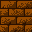
\includegraphics[scale=1]{3Bricks}
  \caption{Bricks Original Pattern}
\end{subfigure}
\caption{Original Input Patterns}
\label{fig:oginput}
\end{figure}

\newpage
\null
\vfill
\begin{figure}[h]
\centering
\begin{subfigure}{.5\textwidth}
  \centering
  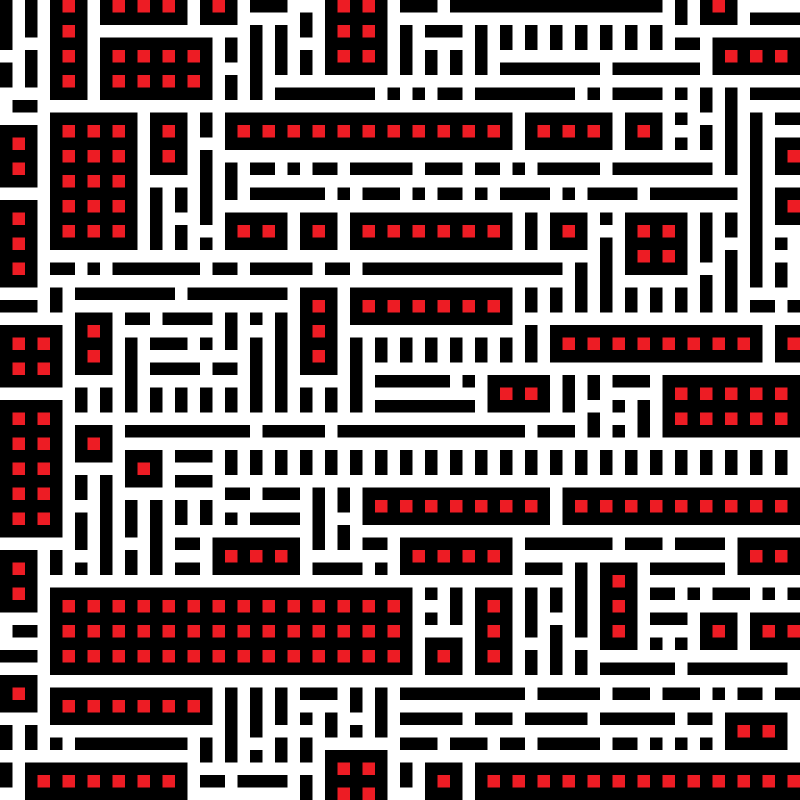
\includegraphics[scale=0.22]{redResultQRNG}
  \caption{Wave Function Collapse with QRNG}
  \label{fig:redqrng}
\end{subfigure}%
\begin{subfigure}{.5\textwidth}
  \centering
  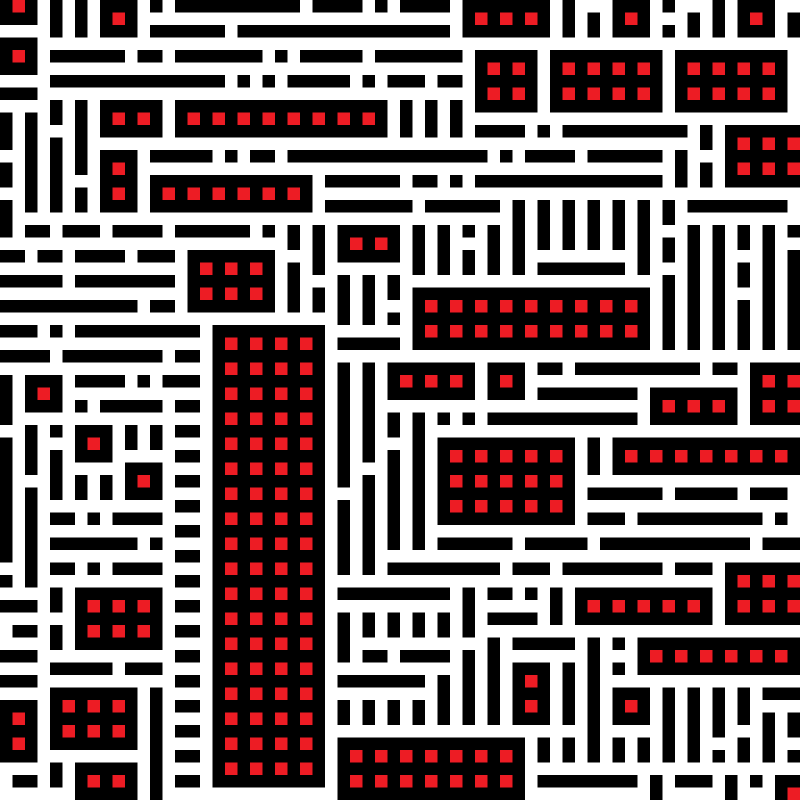
\includegraphics[scale=0.22]{redResultClassical}
  \caption{Classical Wave Function Collapse}
  \label{fig:redclass}
\end{subfigure}
\caption{Comparison of Classical and QRNG Wave Function Collapse for Red Maze Pattern}
\label{fig:redcompare}
\end{figure}
\begin{figure}[h]
\centering
\begin{subfigure}{.5\textwidth}
  \centering
  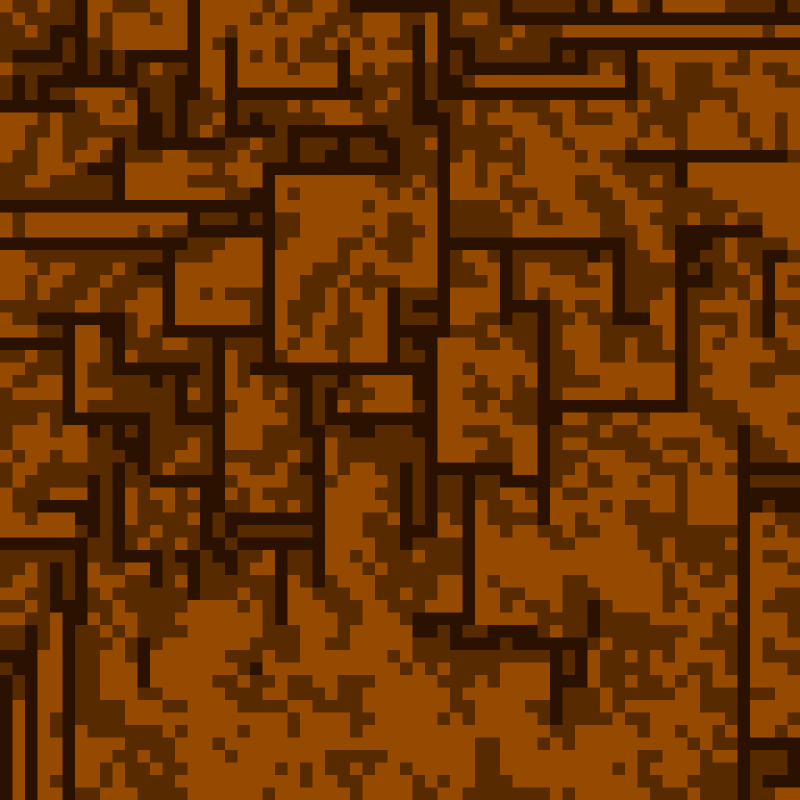
\includegraphics[scale=0.2]{bricksResultQRNG}
  \caption{Wave Function Collapse with QRNG}
  \label{fig:brickqrng}
\end{subfigure}%
\begin{subfigure}{.5\textwidth}
  \centering
  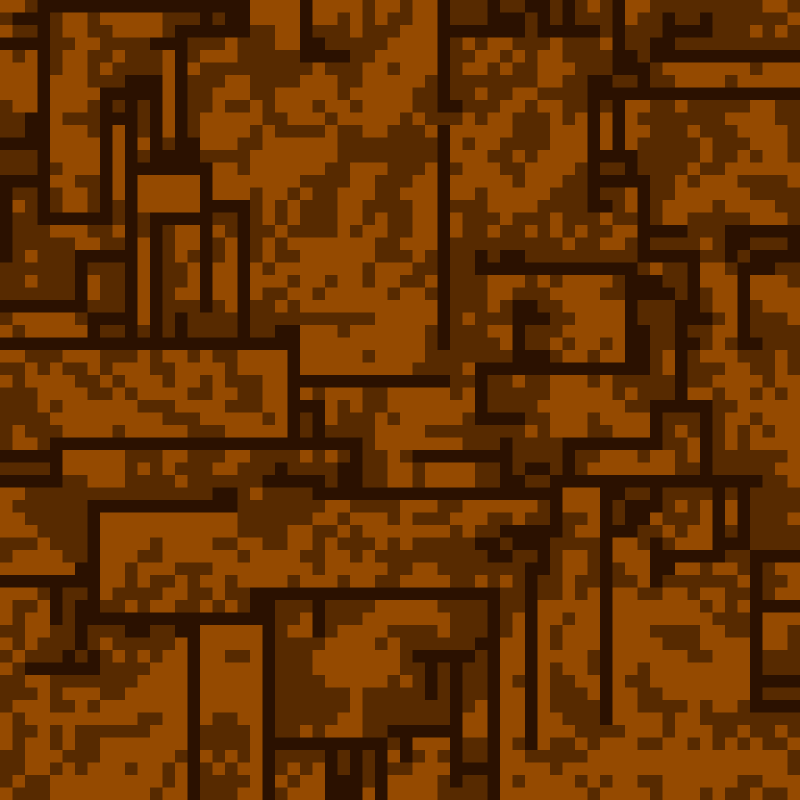
\includegraphics[scale=0.2]{bricksResultClassical}
  \caption{Classical Wave Function Collapse}
  \label{fig:brickclass}
\end{subfigure}
\caption{Comparison of Classical and QRNG Wave Function Collapse for Brick Pattern}
\label{fig:brickcompare}
\end{figure}
\vfill

\newpage
\section{Tests}
The tests we considered were based off of input images provided in the original implementation of the WaveFunctionCollapse algorithm. Given these input images, we can output what our board generated and observe whether or not this output image is locally similar to the original input. The input images are small and indicate which pattern we expect to see in the much larger output image. We considered in total eight input images to test this on.

\end{document}